\chapter{Implementation and Validation}

This section presents our understanding of the implementation of the depression prediction model developed for the Kaggle Playground Series S4E11 competition. The code was written by Mahdi Ravaghi and publicly released as the winning solution. Our goal here is to demonstrate a high-level understanding of how the system operates, how the data was processed, and how the model was validated for its stated objective of maximizing predictive accuracy.

\section{Data Cleaning and Pre-processing}

The original pipeline involved substantial pre-processing to prepare the dataset for machine learning. Categorical features were cast as \texttt{category} dtype, with category alignment enforced across the training and test datasets. For certain models (e.g., AdaBoost and XGBoost), ordinal encoding was applied to categorical variables. Continuous features with missing values were imputed using mean imputation. The final feature matrix was standardized for models that were sensitive to feature scaling (e.g., Logistic Regression and Ridge Regression). Importantly, gender and other categorical fields were preserved as-is to allow downstream auditing of subgroup behavior. The data itself is synthetic, generated from an undisclosed private dataset, and does not include real personal identifiers.

\section{High-level Implementation of the System}

The system follows a stacked ensemble architecture. The first layer (L1) consists of five base models: AdaBoost, CatBoost, XGBoost, LightGBM, and Logistic Regression. Each of these models was trained independently and generated probability outputs on the validation set. These predictions were passed to a second-level ensemble (L2), where two models—Logistic Regression and Ridge Regression—were trained using the logit-transformed probabilities of the base models as inputs. These L2 models effectively learned how to weight the base model predictions. Finally, an L3 ensemble combined the outputs of the L2 models using a weighted average, with the optimal weights learned via hyperparameter tuning (using Optuna). This layered design was intended to maximize accuracy while leveraging the strengths of diverse classifiers.

The original implementation used stratified $k$-fold cross-validation to evaluate model performance and select hyperparameters. This approach is standard in ML competitions and helps ensure robust performance estimates by averaging accuracy across multiple validation splits.

\section{Validation and Alignment with Stated Goals}

The ADS was validated using stratified cross-validation, and the stated goal—maximizing accuracy—was achieved, with the final model reaching approximately 94–96\% average accuracy across folds. However, since the competition’s test set did not contain ground-truth labels, external validation and fairness analysis were not originally conducted. To audit the model for fairness, we created a fixed train-validation split from the training data. This enabled the use of fairness metrics such as selection rate, true/false positive rates, and enabled consistent subgroup analysis via Fairlearn’s \texttt{MetricFrame}.

We also discovered that cross-validation introduces variability in subgroup representation across folds, complicating fairness analysis. A fixed validation set allowed for reproducible and interpretable group-level metrics. Figure~\ref{fig:model_before} shows model performance under cross-validation, and Figure~\ref{fig:model_after} shows performance under our fixed split.

\begin{figure}[H]
\centering
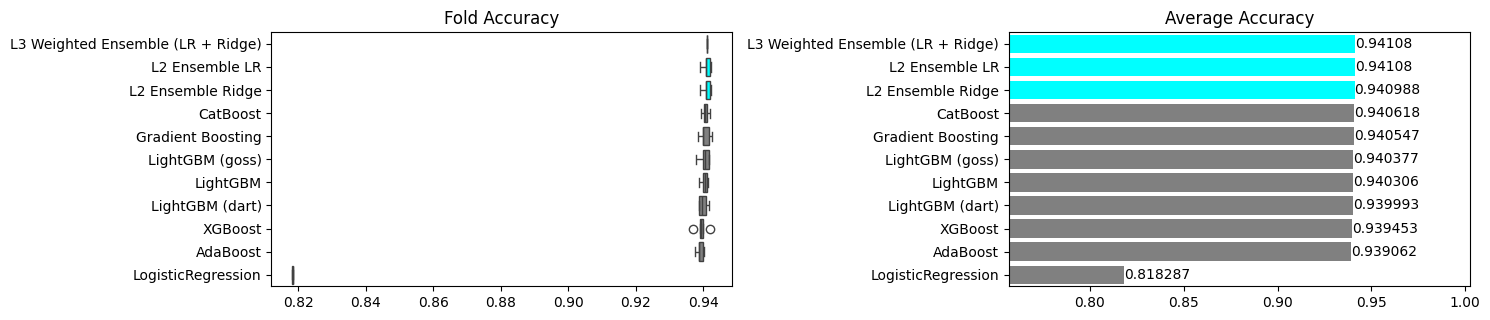
\includegraphics[width=0.87\linewidth]{figures/model_before.png}
\caption{Cross-validated accuracy comparison of different models under the original ensemble pipeline. The L3 weighted ensemble achieves the highest mean accuracy.}
\label{fig:model_before}
\end{figure}

\begin{figure}[H]
\centering
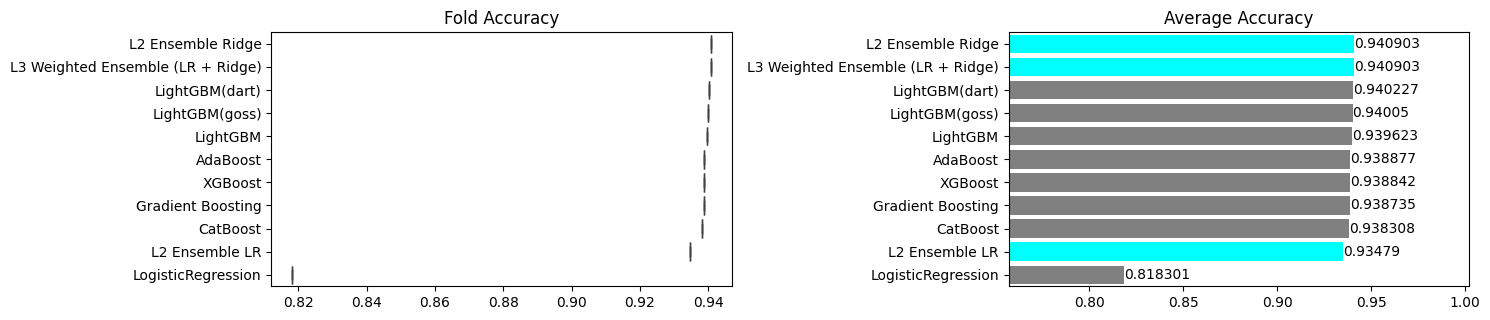
\includegraphics[width=0.87\linewidth]{figures/model_after.png}
\caption{Accuracy comparison of models using a fixed train-validation split. Overall rankings remain consistent, but this approach enables fair and consistent subgroup evaluation.}
\label{fig:model_after}
\end{figure}

That said, our fixed-split strategy may have introduced information leakage or artifacts, as the data is synthetic and its generative process is not fully disclosed. Future work could involve generating privacy-preserving synthetic datasets using differentially private mechanisms or correlation-aware generative models.\\
In summary, the implementation was accurate and sophisticated in terms of ensemble architecture and optimization, but fairness and robustness to distributional shift were not considered in the original validation pipeline. Our re-validation using a fixed split enabled a more thorough fairness audit aligned with the needs of a real-world ADS.